\documentclass[12pt]{report}

\usepackage{amsmath}
\usepackage{amssymb}
\usepackage{graphicx}
\usepackage{framed}

\headsep = 5pt
\footskip = 10pt
\textheight = 672pt
\begin{document}


\section*{Question 2}
\subsection*{Part A : Builder Method}
The following sets have been defined using the \textbf{Building Method} of notation. Re-write them by listing \textbf{some} of the elements.
\begin{enumerate}
\item $\{p | p$ is a capital city, p is in Europe$\}$
\item $\{x | x = 2n - 5,$ x and n are natural numbers$\}$
\item $\{y | 2y^2 = 50,$ y is an integer$\}$
\item $\{z | z = n^3,$ z and n are natural numbers$\}$
\end{enumerate}
\subsection*{Part B : Sets}
U = {natural numbers}; $A = \{2, 4, 6, 8, 10\}$; $B = \{1, 3, 6, 7, 8\}$. State whether each of the following is true or false:
\begin{itemize}
\item[(i)] $A \subset U$
\item[(ii)] $B \subseteq A$
\item[(iii)] $\emptyset \subset U$
\end{itemize}

%-------------------------------------- %

\section*{Question 3}
\subsection*{Part A : Propositions}
Let p, q be the following propositions:
\begin{itemize}
\item p : this apple is red, 
\item q : this apple is ripe.
\end{itemize}

\noindent Express the following statements in words as simply as you can:
\begin{itemize}
\item[(i)] $p \rightarrow q$
\item[(ii)] $p \wedge \neg q$.
\end{itemize}
 
\noindent Express the following statements symbolically:
\begin{itemize}
\item[(iii)] This apple is neither red nor ripe.
\item[(iv)] If this apple is not red it is not ripe.
\end{itemize}

\subsection*{Part B : Logical Operations}
Let $n \in \{1,2,3,4,5,6,7,8,9\}$ and let p and q be the following propostions concerning 
the integers $n$.

\begin{itemize}
\item[p] $n$ is event
\item[q] $n<5$
\end{itemize}

Find the values of $n$ for which each of the following compound statement is true,

\begin{itemize}
\item[(i)] $\neg p$
\item[(ii)] $p \wedge q$
\item[(iii)] $\neg p \vee q$ 
\item[(iv)] $p \oplus q$
\end{itemize}

%------------------------------------%
\newpage
\section*{Question 5}
\begin{enumerate}
\item Draw two non-isomorphic graphs with the following degree sequence.
\[ 4,3,3,2,2,2,2,1,1\]
\item Write out the degree sequence of the following graph.
%\begin{figure}[h!]
%\centering
%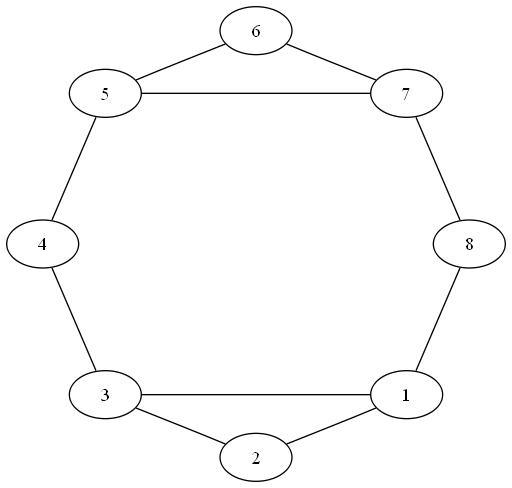
\includegraphics[width=0.5\linewidth]{./graph2.jpg}
%%\caption{}
%\label{fig:graph2}
%\end{figure}
\item State the vertices that comprise a cycle of length 5 in both of the following graphs.
%\begin{figure}[h!]
%\centering
%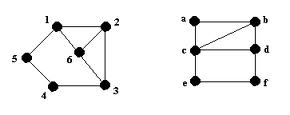
\includegraphics[width=0.7\linewidth]{./graph20.jpg}
%
%\label{fig:graph20}
%\end{figure}
\end{enumerate}
\newpage










%-----------------------------------------------------%
\section*{Question 6}

\subsection*{Part A : Digraphs}

Suppose $A = $$\{1,2,3,4\}$. Consider the following relation in A

\[ \{  (1,1),(2,2),(2,3),(3,2),(4,2),(4,4)\} \]

Draw the direct graph of $A$. Based on the Digraph of $A$ discuss whether or not a relation that could be depicted by the digraph could be described as the following, justifying your answer.


\begin{itemize}
\item[(i)] Symmetric
\item[(ii)] Reflexive 
\item[(iii)] Transitive
\item[(iv)] Antisymmetric
\end{itemize}
\subsection*{Part B : Relations}
Determine which of the following relations $ x R y$ are reflexive, transitive, symmetric, or antisymmetric on the following - there may be more than one characteristic.  if

\begin{itemize} 
\item[(i)] $x = y$
\item[(ii)] $x < y$
\item[(iii)] $x^2 = y^2$
\item[(iv)] $x \geq y$
\end{itemize}
\subsection*{Part C : Partial Orders}
% http://staff.scem.uws.edu.au/cgi-bin/cgiwrap/zhuhan/dmath/dm_readall.cgi?page=20

Let $A=\{0,1,2\}$ and $R=\{ (0,0),(0,1),(0,2),(1,1), (1,2), (2,2)\}$
 and $S=\{(0,0),(1,1),(2,2)\}$ be 2 relations on A. Show that

\begin{itemize}
\item[(i)] R is a partial order relation.
\item[(ii)] S is an equivalence relation.
\end{itemize}


%------------------------------------%
\section*{Question 7}
\subsection*{Part A : Recurrence Relations}
A sequence is defined by the recurrence relations
 \[x_{n+2}  = 3x_{n+1} - 2x_n\]
with initial terms $x_1 = 1$ and $x_2=3$.

\begin{itemize}
\item[(i)] Calculate $x_3$, $x_4$ and $x_5$, showing your workings.
\item[(ii)] Prove by induction that $x_n = 2^n - 1$ for all $n \geq 1$
\end{itemize}

%------------------------------------%
\subsection*{Part B : Summations}

Compute the following summation

\[ \sum^{i=100}_{i=25} i^2 + 3i -5)\]
%------------------------------------%
\section*{Question 8}
\subsection*{Part A : Spanning Trees}
\begin{enumerate}
\item How many edges are in the spanning tree $T$ ?
\item What is the sum of the degree sequence of $T$?
\item Write down all the possible degree sequences for the spanning tree $T$.
\end{enumerate}
%------------------------------------%

\subsection*{Part B : Binary Search Trees}
Suppose a database, comprised of 30,000 internal nodes, is structured as a Binary Search Tree.

\begin{enumerate}
\item What is the key (number) of the Root node?
\item What are the keys of the nodes at level 1?
\item For the nodes at level1, how many subtrees are there?
\item State which nodes are in the substrees of the level 1 nodes?
\item How many nodes are the between the root (level 0) and level 7. ]
(Hint: use a summation theorem mentioned in session 7
\item What is the maximum number of searchs in this database?
\end{enumerate}
%------------------------------------%
\end{document}